\documentclass[11pt,a4paper]{article}
\usepackage[T1]{fontenc}
\usepackage[spanish,es-nodecimaldot]{babel}
\usepackage[margin=18mm]{geometry}
\usepackage{graphicx,amsmath,booktabs,tabularx,pdfpages}
\graphicspath{{../release/}}
\usepackage[hidelinks]{hyperref}
\hypersetup{pdftitle={Anexo de hardware: convertidor Buck},pdfauthor={Martín Ramírez Espinosa, Jerónimo Vargas Orozco, Andrew Esteban Henao Becerra, Mateo Alexander Cardenas Cuesta}}
\setlength{\parindent}{0pt}
\setlength{\parskip}{6pt}
\begin{document}
\special{pdf:minorversion 7}
\begin{center}
{\LARGE Anexo de hardware: convertidor Buck}\par
{\large Revisión A: diseño preparado; ensayos físicos pendientes}\par
Martín Ramírez Espinosa; Jerónimo Vargas Orozco\\
Andrew Esteban Henao Becerra; Mateo Alexander Cardenas Cuesta\\
Universidad Nacional de Colombia, Sede Manizales
\end{center}
\section*{Alcance y estado}
Este anexo acompaña las cuatro entregas IEEE. Las vistas proceden de la placa KiCad; no son fotografías de un prototipo. La placa tiene 99 por 99 mm, dos capas y 57 componentes. No se han comprado componentes ni realizado ensayos físicos. La fabricación permanece retenida hasta calificar componentes y validar un prototipo soldado.
\begin{center}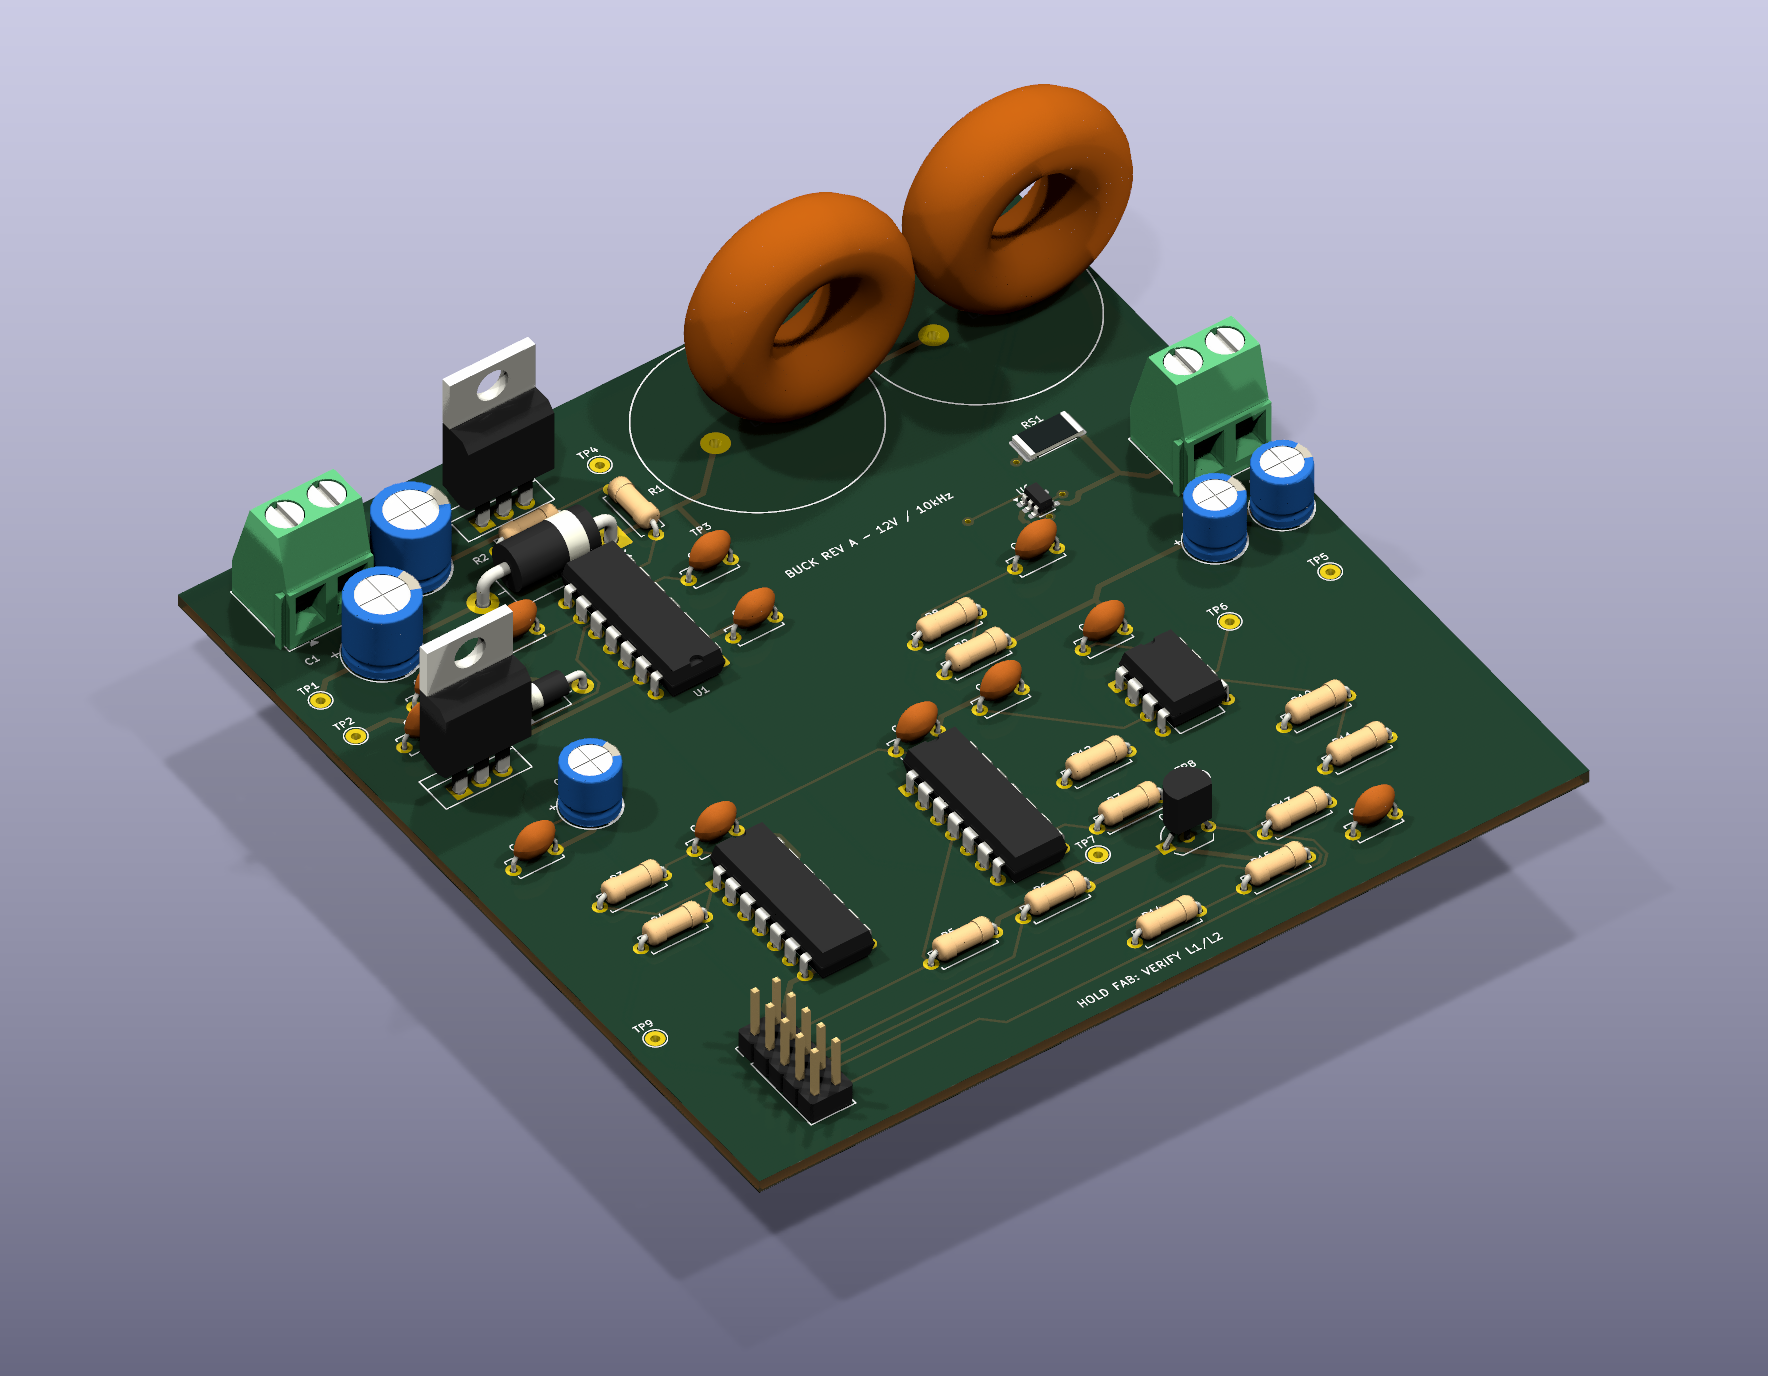
\includegraphics[width=.9\linewidth]{report-assets/pcb-3d.png}\end{center}
\textbf{Figura 1.} Vista CAD isométrica. Los encapsulados estándar proceden de la biblioteca oficial KiCad. L1/L2 usan envolventes provisionales de 25 mm de diámetro: no representan dimensiones verificadas, bobinado ni terminales comerciales. Los capacitores representan el encapsulado previsto, con referencia y altura comercial pendientes. El MCU y accesorios son externos. Las vistas no certifican holguras, disipación ni montaje.

\newpage
\section*{Vista superior y localización}
\begin{center}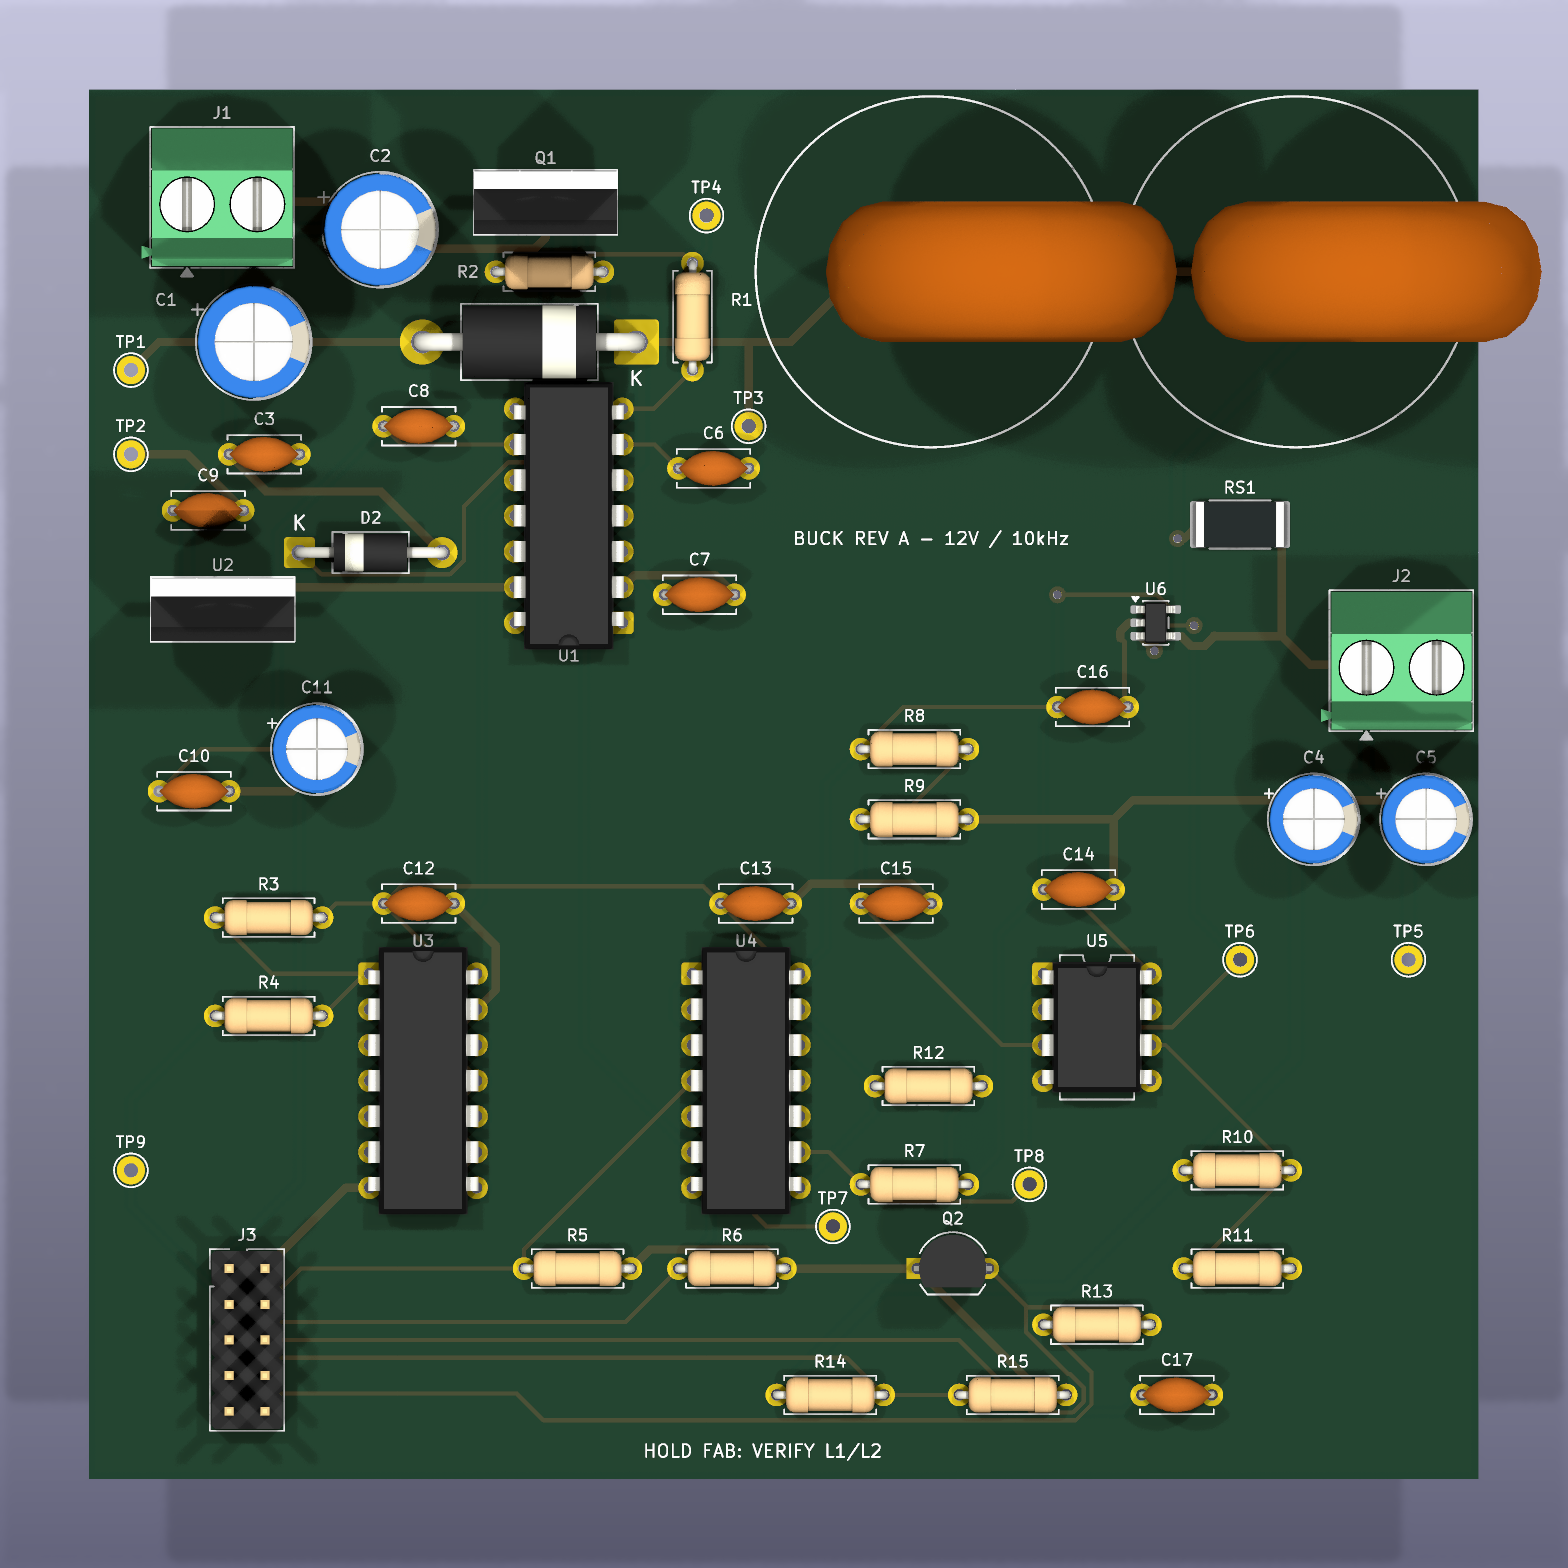
\includegraphics[width=.79\linewidth]{report-assets/pcb-top.png}\end{center}
\textbf{Figura 2.} Vista superior CAD. La posición corresponde al archivo de placa. Verificar orientación, polaridad y dimensiones contra las piezas recibidas antes de ordenar.
\par
\begin{tabularx}{\linewidth}{lX}
\toprule Referencias & Función \\\midrule
J1; J2; J3 & Entrada con fusible externo; salida a carga; interfaz MCU.\\
Q1; D1; L1/L2; RS1 & MOSFET; rueda libre; inductancia serie; shunt.\\
U1; U2; U3 & IR2110; regulador 5 V; inversor HCT14.\\
U4; U5; U6 & Enclavamiento HCT00; comparadores LM393; INA180A1.\\
C4/C5 & Dos capacitores de 10 $\mu$F en paralelo.\\\bottomrule
\end{tabularx}

\newpage
\section*{Plano de componentes}
\begin{center}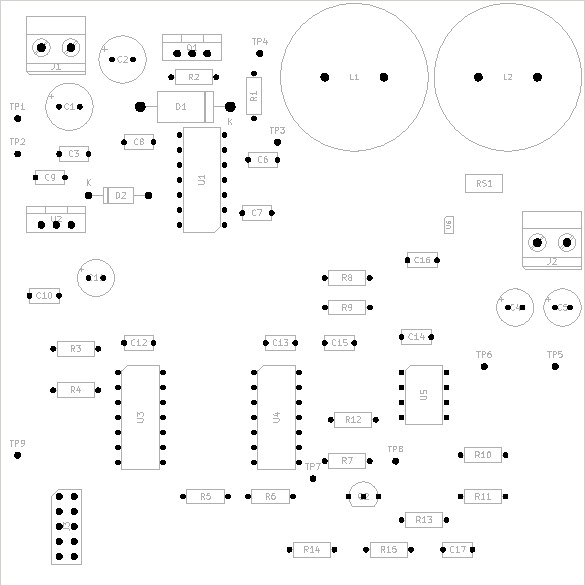
\includegraphics[width=\linewidth,height=.78\textheight,keepaspectratio]{report-assets/layout.pdf}\end{center}
\textbf{Figura 3.} Plano vectorial de referencias, contornos y pads exportado desde KiCad. Las vistas 3D y este plano son complementarios. La envolvente provisional de L1/L2 no autoriza fabricación.

\newpage
\section*{Interconexión y puntos de medida}
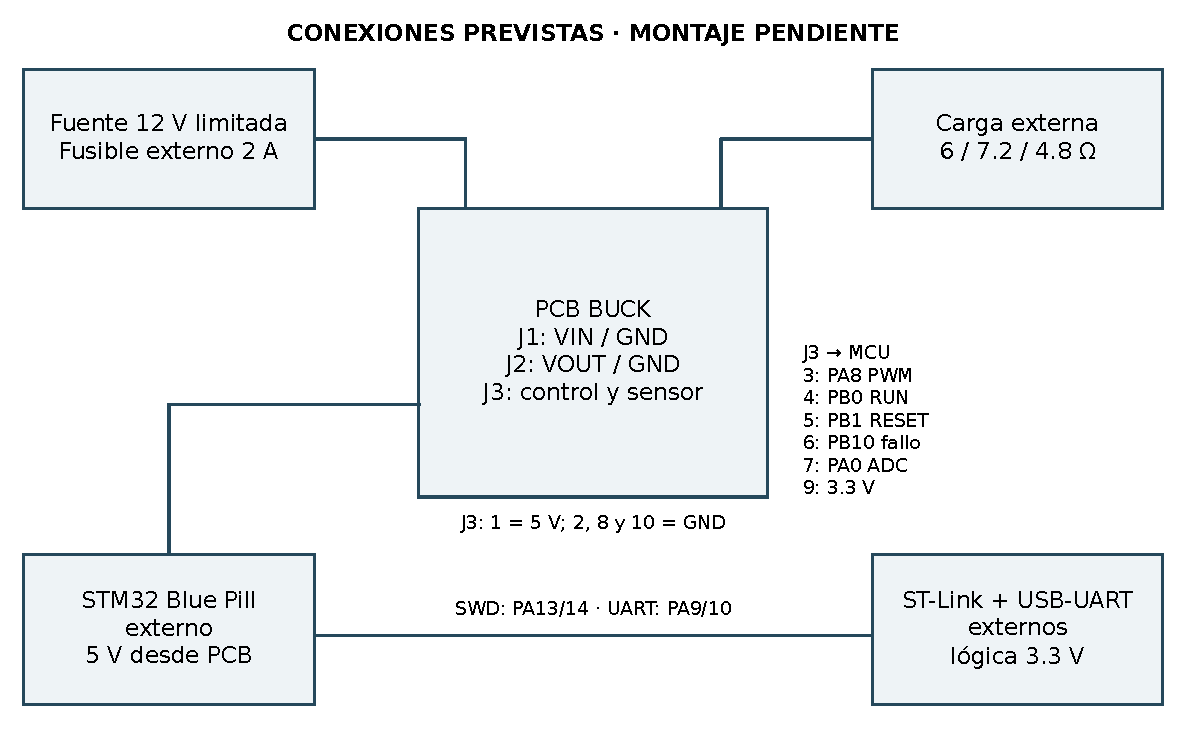
\includegraphics[width=\linewidth]{report-assets/wiring.pdf}
\par
\begin{tabularx}{\linewidth}{lX}
\toprule Punto & Medida prevista \\\midrule
TP1 / TP2 & VIN / GND.\\
TP3 / TP4 & SW / GATE; $v_{GS}=V(\mathrm{TP4})-V(\mathrm{TP3})$, medida diferencial.\\
TP5 / TP6 & VOUT / ISENSE (nominalmente 1 V/A).\\
TP7 / TP8 / TP9 & SD / NTRIP / PWM $d'$.\\\bottomrule
\end{tabularx}\par
J3: 1 = 5 V; 2, 8, 10 = GND; 3 = PA8; 4 = PB0; 5 = PB1; 6 = PB10 (fallo activo bajo); 7 = PA0; 9 = 3.3 V desde MCU. Conectar con alimentación apagada. Evitar realimentación entre USB, programador y reguladores. Verificar si el pin de 3.3 V del ST-Link es salida de alimentación o referencia; no unir fuentes independientes.

\section*{Apagado y enclavamiento}
\begin{tabularx}{\linewidth}{ccccX}
\toprule NTRIP & RESET & RUN & SD & Resultado \\\midrule
0 & X & X & 1 & Disparo prioritario; fallo enclavado.\\
1 & 0 & 0 & 1 & Salida deshabilitada; conserva fallo previo.\\
1 & 1 & 0 & 1 & Limpia fallo con salida deshabilitada.\\
1 & 0 & 1 & 0/1 & Habilita sólo si no hay fallo enclavado.\\\bottomrule
\end{tabularx}\par
Umbrales nominales: 2 A y 8.2 V. Intervalos estáticos calculados: 1.825--2.184 A y 7.561--8.868 V. No incluyen la verificación experimental del retardo ni garantizan ausencia de sobrepicos. Nunca conectar la masa de una sonda convencional al nodo SW.

\newpage
\section*{Revisión contra la guía original}
\begin{tabularx}{\linewidth}{lXX}
\toprule Entrega & Requisito y evidencia disponible & Trabajo pendiente \\\midrule
1 (20\%) & Derivación, dinámica, dos escalones de $d'$ y errores; MATLAB/Simulink y circuito ngspice. & Revisión docente del informe; el circuito BJT no es la placa IR2110.\\
2 (30\%) & PCB, lista de materiales, captura y protocolo preparados. & Montaje funcional; medir RLC; ajustar modelo; dos escalones físicos y errores.\\
3 (20\%) & Especificaciones, PI por respuesta en frecuencia, cuatro casos numéricos; estimación PCB adicional separada. & Confirmar aceptación de la ubicación elegida del cero respecto a la recomendación de clase.\\
4 (30\%) & Firmware ARM compilado, pruebas C y captura, protocolo de cuatro casos. & Programar MCU, calibrar, medir temporización/protecciones, cuatro pruebas físicas y reajuste si procede.\\\bottomrule
\end{tabularx}\par
La lámina 90 del capítulo 10 recomienda normalmente cero PI por debajo del cruce. La entrega 3 explica por qué se escogió 3000 rad/s con cruce de 1000 rad/s y comprueba su margen; no se afirma seguir literalmente esa recomendación. Los porcentajes son pesos de evaluación, no porcentaje ganado ni avance calculado. Las fechas de mayo de 2025 de la guía deben confirmarse para el curso actual.

\section*{Secuencia de trabajo del equipo}
\begin{enumerate}
\item Cerrar referencias, disponibilidad y dimensiones; medir o conseguir datos de DCR, saturación y rizado admisible. Objetivo COP 350\,000; estimado COP 281\,501.95 con asignaciones de transporte y reserva COP 68\,498.05, sin cotización final entregada.
\item Obtener y verificar MCU y componentes. Validar prototipo soldado con fuente limitada: inversión, bootstrap, apagado, protección y sensores.
\item Corregir el diseño según evidencia. Repetir ERC/DRC y comparar cotizaciones entregadas de PCBWay y JLCPCB; liberar fabricación sólo tras resolver bloqueos.
\item Fabricar, montar e inspeccionar. Medir RLC y calibrar ADC con dos puntos, comprobar con un tercero; medir PWM, latencia, rizado y temperatura.
\item Ejecutar tres repeticiones de los dos casos abiertos y los cuatro cerrados: 18 registros mínimos. Usar osciloscopio para rizado y pretrigger en carga.
\item Incorporar capturas, parámetros reales, incertidumbre y errores en entregas 2 y 4. Conservar datos previos a cualquier reajuste.
\end{enumerate}

\section*{Fuentes y trazabilidad}
Guía: \emph{Descripción Proyecto Buck}, pp. 1--3. Método: \emph{10 The Frequency-Response Design Method}, sección 7. Archivos KiCad y manifiesto de modelos en \texttt{project/pcb}; hojas de datos y enlaces en \texttt{docs/sources.md}. Simulación adicional en \texttt{release/simulation}. Los esquemas completos siguen en cinco páginas vectoriales exportadas directamente desde KiCad; ampliar para consultar pines y redes.
\newpage
\section*{Conectividad resumida de la etapa de potencia}
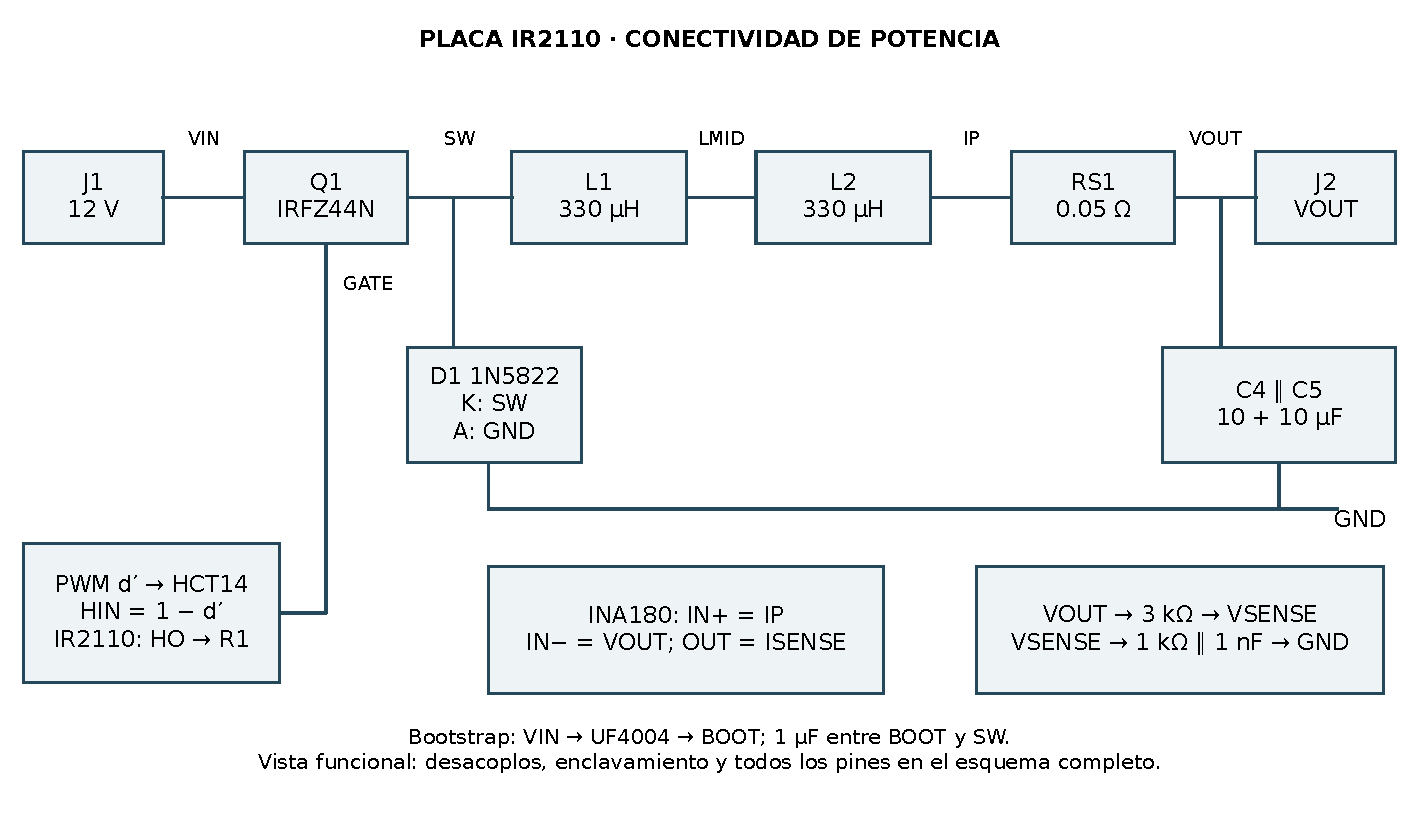
\includegraphics[width=\linewidth]{report-assets/power-summary.pdf}

\textbf{Figura 4.} Vista funcional de las redes de potencia y del signo de la entrada. L1 y L2 están en serie; RS1 está entre IP y VOUT. C4 y C5 comparten VOUT y GND. El esquema completo de las páginas siguientes detalla todos los pines, desacoplos, alimentación y protección. Esta vista no debe usarse sola para ensamblar.
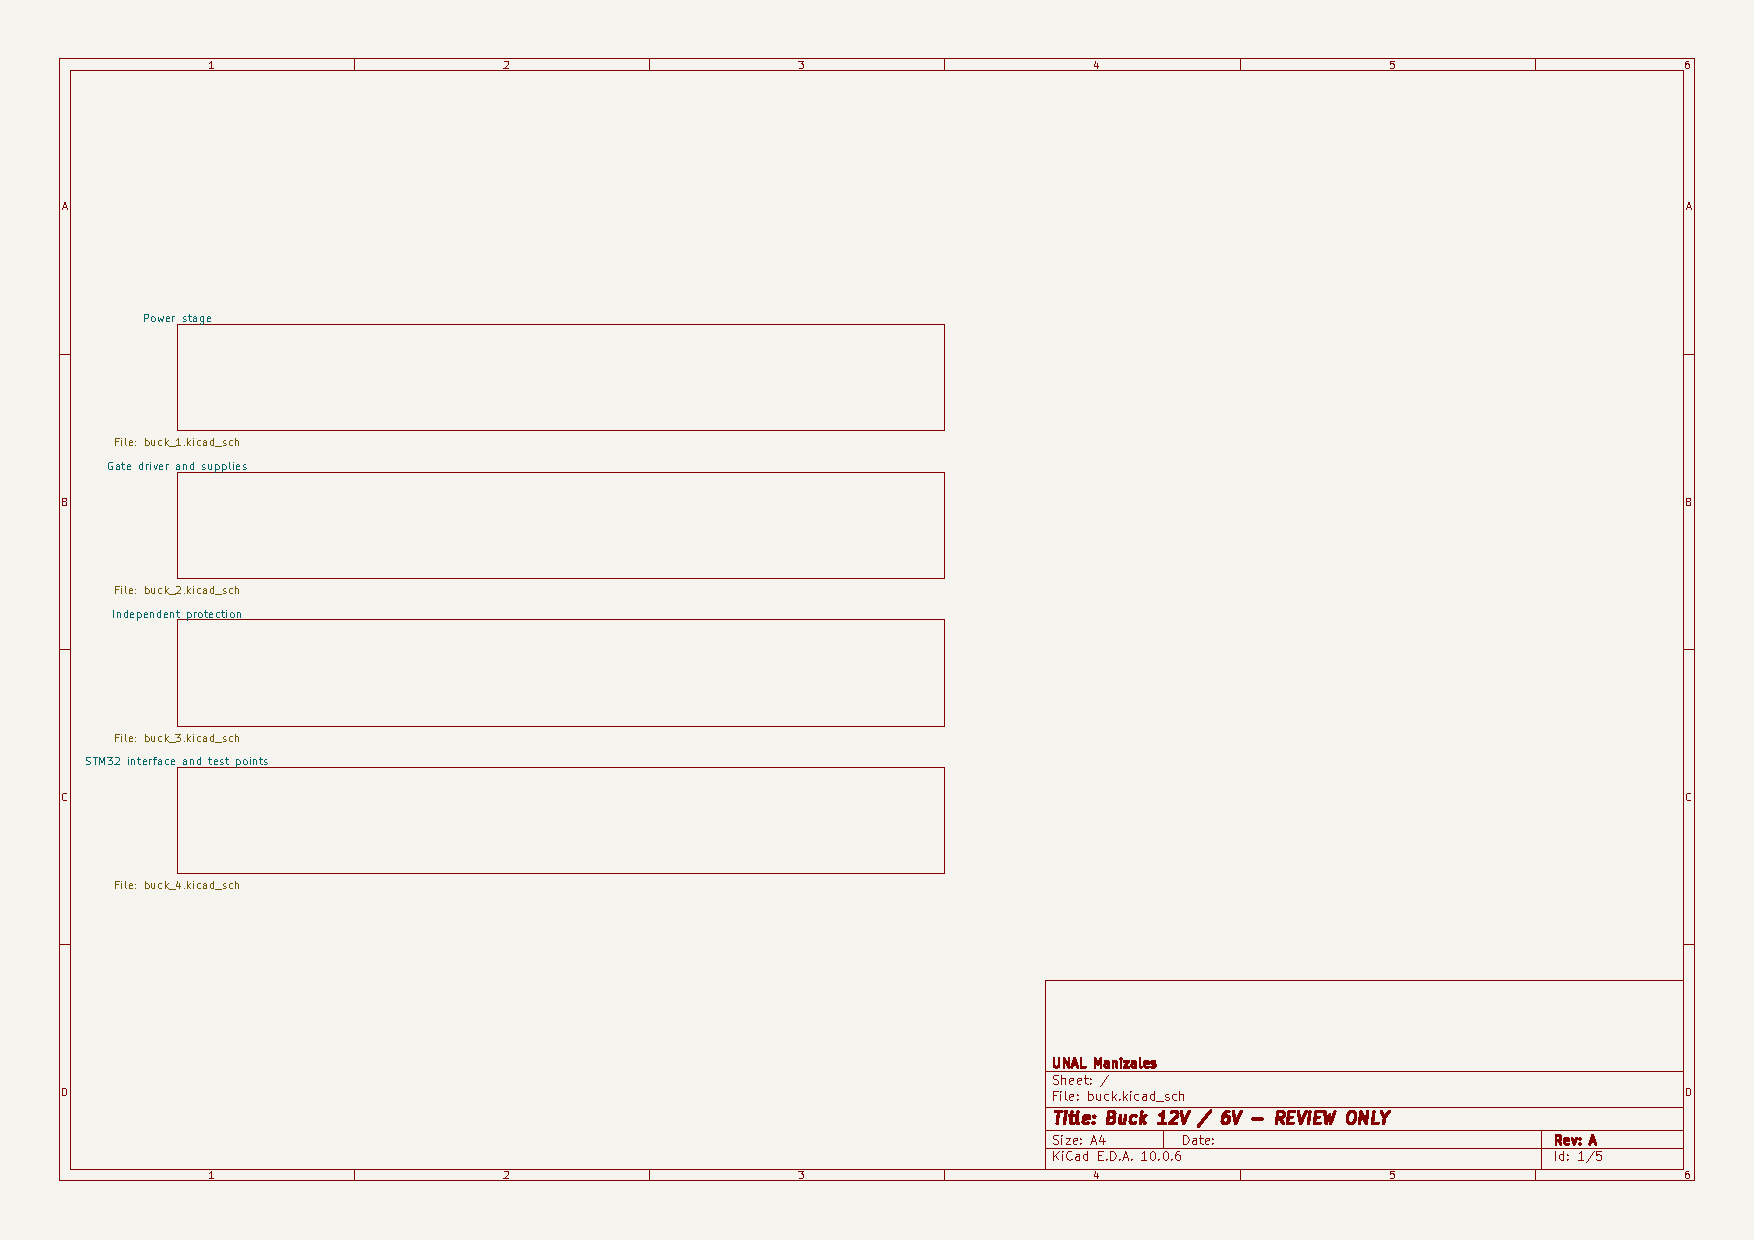
\includepdf[pages=-,fitpaper=true]{../release/schematic.pdf}
\end{document}
